\documentclass[12pt]{article}
\usepackage{graphicx}
\usepackage{xcolor}
\usepackage{geometry}
\geometry{margin=1in}

\begin{document}

\begin{center}
\includegraphics[width=0.3\textwidth]{images/logo.jpg}
\end{center}

\begin{center}
\textbf{\Large Harshita N Kumar} \\
\textbf{ID: COMETFWC052}
\end{center}

\vspace{0.5cm}

\begin{center}
{\color{blue}\Huge GATE Question No. 41}
\end{center}

\vspace{0.5cm}

{\color{blue}\Large Question}

\vspace{0.3cm}

\includegraphics[width=\textwidth]{images/question.jpg}

\vspace{0.5cm}

{\color{blue}\Large Given Circuits}

\vspace{0.3cm}

\includegraphics[width=\textwidth]{images/gates.jpg}

\vspace{0.5cm}

{\color{blue}\Large Question Analysis}

The circuits (a), (b), and (c) simplify to:

$Q = A\overline{B}$

Circuit (d) simplifies to:

$Q = \overline{A} + B$

Since the expressions are different, option (d) is the incorrect circuit.

\vspace{0.5cm}

{\color{blue}\Large Truth Table}

\begin{center}
\begin{tabular}{|c|c|c|}
\hline
A & B & Q = A\overline{B} \\
\hline
0 & 0 & 0 \\
0 & 1 & 0 \\
1 & 0 & 1 \\
1 & 1 & 0 \\
\hline
\end{tabular}
\end{center}

\vspace{0.5cm}

{\color{blue}\Large Hardware Implementation}

The function implemented is:

$Q = A\overline{B}$

Arduino and 7447 are used to display the output.

\vspace{0.5cm}

{\color{blue}\Large Required Components}

\begin{itemize}
\item Arduino UNO
\item IC 7447
\item Common Anode 7-segment display
\item Resistors
\item Breadboard
\item Jumper wires
\end{itemize}

\vspace{0.5cm}

{\color{blue}\Large Pin Connections}

\begin{itemize}
\item Arduino Pin 10 $\rightarrow$ Input A
\item Arduino Pin 11 $\rightarrow$ Input B
\item Arduino Pin 9 $\rightarrow$ 7447 Pin 7
\item 7447 Pin 16 $\rightarrow$ 5V
\item 7447 Pin 8 $\rightarrow$ GND
\item 7447 Pins 3,4,5 $\rightarrow$ 5V
\item 7447 Pins 1,2,6 $\rightarrow$ GND
\item 7-segment common pins $\rightarrow$ 5V
\end{itemize}

\vspace{0.5cm}

{\color{blue}\Large Code Uploading Steps}

\begin{enumerate}
\item Create a Platform IO project.
\item Write the code in main.cpp inside src folder.
\item Run the command "pio run".
\item Copy the generated .hex file to Arduino Droid folder.
\item Connect Arduino UNO to mobile using OTG cable.
\item Upload the hex file using "upload precompiled" option.
\item Observe the output and verify the expression.
\end{enumerate}

\vspace{0.5cm}

{\color{blue}\Large Experimental Truth Table}

\begin{center}
\begin{tabular}{|c|c|c|}
\hline
A & B & Displayed Output \\
\hline
0 & 0 & 0 \\
0 & 1 & 0 \\
1 & 0 & 1 \\
1 & 1 & 0 \\
\hline
\end{tabular}
\end{center}

\vspace{0.5cm}

{\color{blue}\Large Hardware Setup}

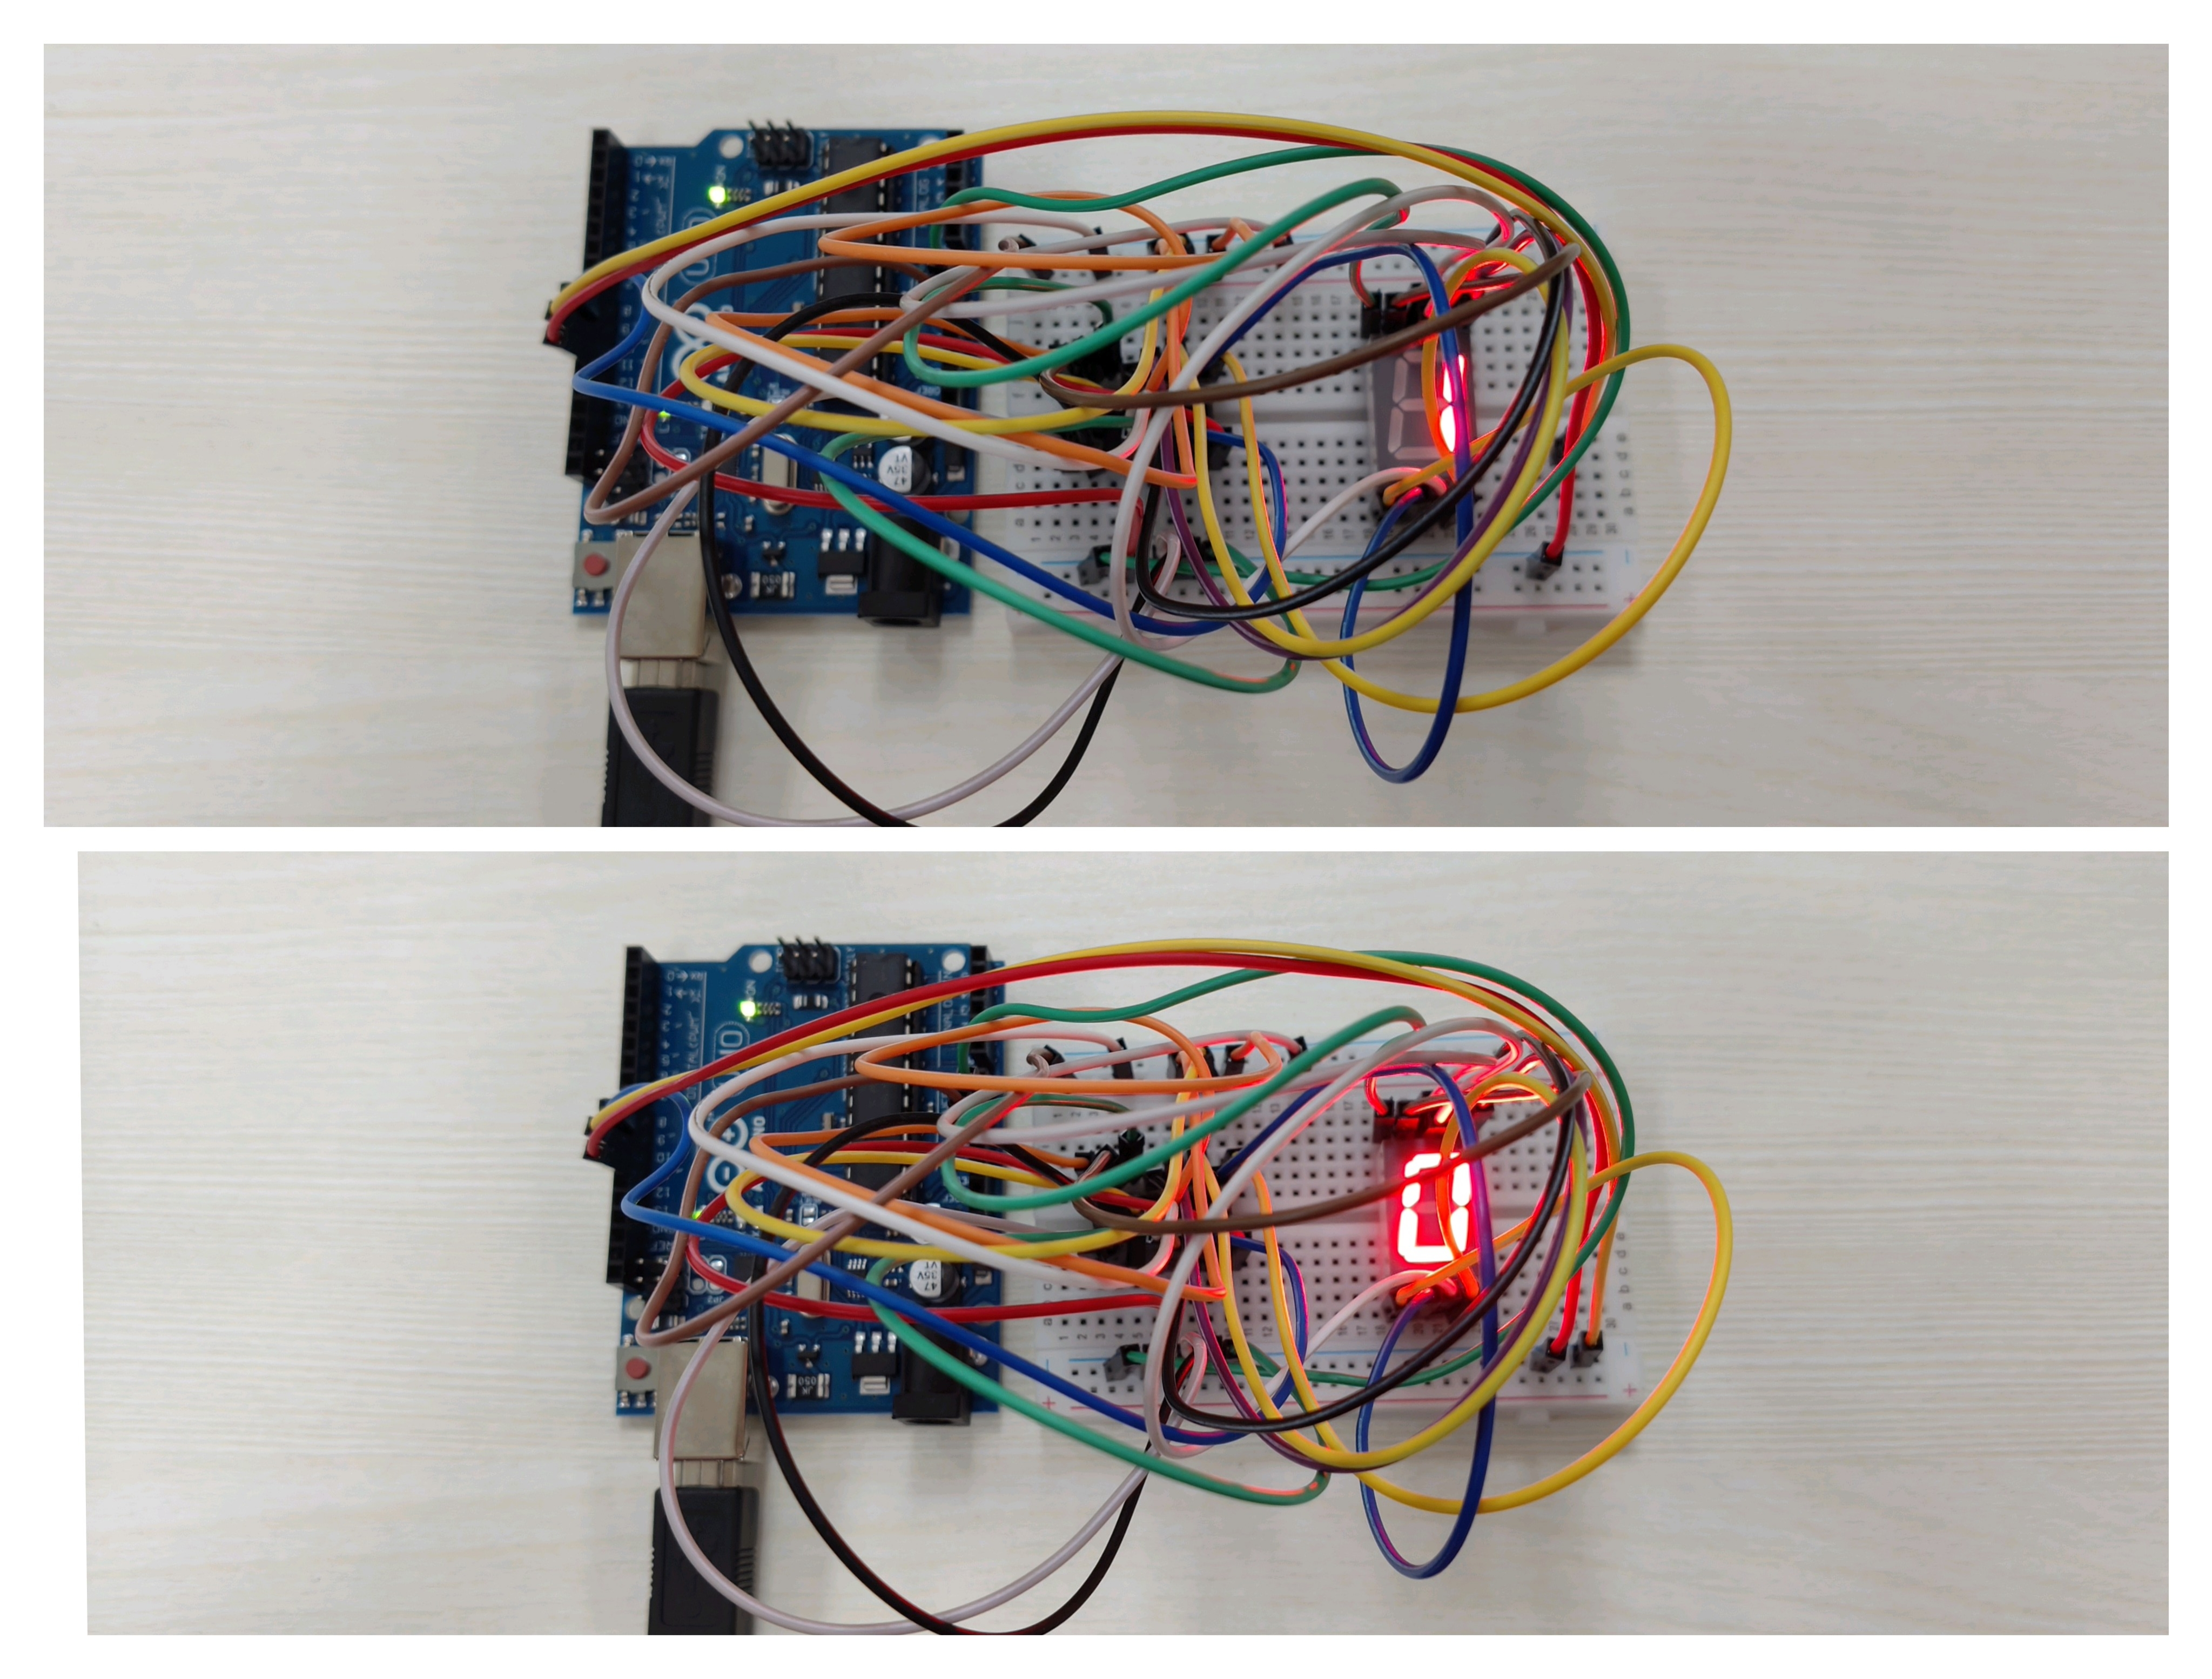
\includegraphics[width=\textwidth]{images/hardware.jpg}

\vspace{0.5cm}

{\color{blue}\Large Conclusion}

From Boolean simplification and hardware verification, circuits (a), (b), and (c) implement $Q = A\overline{B}$.

Circuit (d) implements $Q = \overline{A} + B$.

Therefore, option (d) is the incorrect circuit.

\end{document}
